\documentclass[11pt, titlepage]{article}

\usepackage[letterpaper, hmargin=1in, bmargin=1in, tmargin=1.3in,
headheight=26pt]{geometry}

\usepackage{graphicx}
\usepackage{hyperref}
\usepackage{array}
\newcolumntype{C}[1]{>{\centering\arraybackslash}m{#1}}
\newcolumntype{N}[1]{>{\centering\arraybackslash}p{#1}}
\usepackage{longtable}
\usepackage{multirow}
\usepackage{tabularx}
\usepackage{float}
\usepackage{booktabs}
\usepackage[usenames,dvipsnames,table]{xcolor}
\usepackage{txfonts}
\usepackage[shortcuts]{extdash}

\usepackage[nottoc,notlof,notlot,numbib]{tocbibind}

\usepackage{natbib}

\usepackage[page]{totalcount}

\usepackage{fancyhdr}
\fancyhf{}
\lhead{Module Guide \\ \progname{}}
\rhead{Geneva M. Smith \\ Dept. of Computing and Software---McMaster University}
\lfoot{Ver.~\ref{current_version_MG}}
\rfoot{\thepage\ of \thepagesMG}

\renewcommand{\footrule}{\vbox to 0pt
    {\makebox[\textwidth]{\hrulefill}\vss}}

\hypersetup{
    bookmarks=true,
    colorlinks=true,
    linktoc=all,
    linkcolor=Purple,
    citecolor=ForestGreen,
    filecolor=WildStrawberry,
    urlcolor=Cerulean
}

\newcommand{\citepg}[2]{\citeauthor{#1}, \citeyear{#1}, p.~#2}

\makeatletter
\newcommand\newref[1]{#1\def\@currentlabel{#1}}
\makeatother

%% Comments

\usepackage{color}

\newif\ifcomments\commentstrue

\ifcomments
\newcommand{\authornote}[3]{\textcolor{#1}{[#3 ---#2]}}
\newcommand{\todo}[1]{\textcolor{red}{[TODO: #1]}}
\else
\newcommand{\authornote}[3]{}
\newcommand{\todo}[1]{}
\fi

\newcommand{\wss}[1]{\authornote{blue}{SS}{#1}}
\newcommand{\wgs}[1]{\authornote{teal}{GS}{#1}}
\newcommand{\wjc}[1]{\authornote{purple}{JC}{#1}}

\usepackage{xr}
\externaldocument{../../SRS/EMgine_SRS}
\newcommand{\rref}[1]{SRS-R\ref{#1}}
\newcommand{\nfref}[1]{SRS-NF\ref{#1}}
\newcommand{\tyref}[1]{SRS-TY\ref{#1}}
\newcommand{\iref}[1]{SRS-IM\ref{#1}}
\newcommand{\lcref}[1]{SRS-LC\ref{#1}}

\newcounter{acnum}
\newcommand{\actheacnum}{AC\theacnum}
\newcommand{\acref}[1]{AC\ref{#1}}

\newcounter{ucnum}
\newcommand{\uctheucnum}{UC\theucnum}
\newcommand{\uref}[1]{UC\ref{#1}}

\newcounter{mnum}
\newcommand{\mthemnum}{M\themnum}
\newcommand{\mref}[1]{M\ref{#1}}

\newcommand{\progname}{EMgine} % PUT YOUR PROGRAM NAME HERE

\newcommand{\conceptVersion}{1.0}
\newcommand{\srsVersion}{1.5.1}
\newcommand{\mgversion}{1.5}
\newcommand{\misversion}{0.1.1}
\newcommand{\codeversion}{0.1}
\newcommand{\mastertestplanVersion}{1.0}
\newcommand{\verifytestplanVersion}{1.0}
\newcommand{\validatetestplanVersion}{1.0}
\newcommand{\manualversion}{?}

\newcommand{\timetype}{\mathbb{T}}
\newcommand{\deltatimetype}{\mathbb{T}_{\Delta}}
\newcommand{\energytype}{\mathbb{J}}
\newcommand{\energychangetype}{\mathbb{J}_{\Delta}}
\newcommand{\stringtype}{\text{String}}
\newcommand{\emotionintensitytype}{\mathbb{I}}
\newcommand{\responsestrength}{\mathbb{I}_{\Delta}}
\newcommand{\emotionstatetype}{\mathbb{ES}}
\newcommand{\emotionstatedecaytype}{\mathbb{ES}_\lambda}
\newcommand{\emotiontype}{\mathbb{E}}
\newcommand{\emotionkindstype}{\mathbb{K}}
\newcommand{\emotionequilibriumtype}{\mathbb{ES_{\rightleftharpoons}}}
\newcommand{\emotiondecaytype}{\mathbb{I_{\lambda}}}
\newcommand{\egotype}{\mathbb{O}}
\newcommand{\egoidentitytype}{\mathbb{ID}}
\newcommand{\goaltype}{\mathbb{G}}
\newcommand{\plantype}{\mathbb{P}}
\newcommand{\padpoint}{P_{\left(P,A,D\right)}}
\newcommand{\goallabeltype}{\mathbb{L}}
\newcommand{\worldtype}{\mathbb{W}}
\newcommand{\worldstatetype}{\mathbb{S}}
\newcommand{\worldstatechangetype}{\mathbb{S}_{\Delta}}
\newcommand{\statedistancetype}{\mathbb{D}}
\newcommand{\statedistancechangetype}{\mathbb{D}_{\Delta}}
\newcommand{\indexsettype}{\mathbb{IS}}
\newcommand{\goalegotype}{\mathbb{GE}}
\newcommand{\socialrelationtype}{{R^{S}}}
\newcommand{\socialattachmenttype}{\mathbb{SA}}
\newcommand{\actiontype}{\mathbb{AC}}
\newcommand{\actortype}{\mathbb{A}}
\newcommand{\attentiontype}{\mathbb{AT}_x}
\newcommand{\probabilitytype}{\left[0,1\right]}
\newcommand{\maxval}{\mathsf{MAX}}
\newcommand{\True}{\mathit{True}}
\newcommand{\False}{\mathit{False}}
\newcommand{\defEq}{\text{ } \mathlarger{\mathlarger\circeq} \text{ }}

\newcommand{\mOtherChange}{\mathit{otherChange}}
\newcommand{\mActor}{\mathit{actor}}
\newcommand{\mDeliberate}{\mathit{deliberate}}
\newcommand{\mImportance}{\mathit{importance}}
\newcommand{\mFear}{\mathtt{Fear}}
\newcommand{\mAnger}{\mathtt{Anger}}
\newcommand{\mSadness}{\mathtt{Sadness}}
\newcommand{\mJoy}{\mathtt{Joy}}
\newcommand{\mInterest}{\mathtt{Interest}}
\newcommand{\mSurprise}{\mathtt{Surprise}}
\newcommand{\mDisgust}{\mathtt{Disgust}}
\newcommand{\mTrust}{\mathtt{Acceptance}}
\newcommand{\mStore}{\mathit{Store}}
\newcommand{\mControl}{\mathit{Control}}
\newcommand{\mGenerate}{\mathit{Generate}}
\newcommand{\mDecay}{\mathit{Decay}}
\newcommand{\mAppraisal}{\mathit{Appraisal}}

\usepackage[shortlabels, inline]{enumitem}

\begin{document}

    \newcounter{pagesMG}
    \setcounter{pagesMG}{\totalpages}
    % Subtracts one from the total page count so that it does not include the
    % title page
    %\addtocounter{pagesMG}{-1}

    \begin{titlepage}
        \thispagestyle{empty}

        \title{Module Guide for \progname{}: A Computational Model of Emotion
        for
        Enhancing Non-Player Character Believability in Games}
        \author{Geneva M. Smith}
        \date{October 15, 2022}

        \maketitle
    \end{titlepage}

    \pagestyle{fancy}

    \vspace*{\fill}
    \section*{Revision History}
    \begin{center}
        \begin{tabular}{m{0.16\linewidth}C{0.15\linewidth}m{0.59\linewidth}}
            \toprule {\bf Date} & {\bf Version} & {\bf Notes}\\
            \midrule

            \vspace*{1mm}October 15, 2022 &
            \vspace*{1mm}\newref{1.0}\label{current_version_MG} & \vspace*{6mm}
            \begin{itemize}[noitemsep, nosep, leftmargin=*]
                \item Completed First Version based on SRS Version~1.0
            \end{itemize} \\ \midrule

            \vspace*{1mm}July 21, 2022 & \vspace*{1mm}0.8 & \vspace*{6mm}
            \begin{itemize}[noitemsep, nosep, leftmargin=*]
                \item Module decomposition and definition based on SRS
                Version~0.5
                \item Missing references to Non-Functional Requirements in
                Section~\ref{SecConnection}
            \end{itemize} \\
            \bottomrule
        \end{tabular}
    \end{center}
    \vspace*{\fill}

    \clearpage

    \tableofcontents

    \clearpage

    \listoftables

    \listoffigures

    \clearpage

    \section{Symbols, Abbreviations and Acronyms}\label{sec:refs}
For \progname{}'s other symbols, abbreviations, and acronyms, see the:
\begin{itemize}
    \item Software Requirement Specification (SRS) at
    \href{https://github.com/GenevaS/EMgine/blob/main/docs/SRS/EMgine_SRS.pdf}{https://github.com/GenevaS/EMgine/blob/
        \newline main/docs/SRS/EMgine\_SRS.pdf}, and
    \item Module Guide (MG) at
    \href{https://github.com/GenevaS/EMgine/blob/main/docs/Design/MG/EMgine_MG.pdf}{https://github.com/GenevaS/EMgine/blob/main/docs/Design/\newline
        MG/EMgine\_MG.pdf}, and
    \item Module Interface Specification (MIS) at
    \href{https://github.com/GenevaS/EMgine/blob/main/docs/Design/MIS/EMgine_MIS.pdf}{https://github.com/GenevaS/EMgine/blob/main/
        \newline docs/Design/MIS/EMgine\_MIS.pdf}.
\end{itemize}

\begin{center}

    \renewcommand{\arraystretch}{1.2}
    \begin{tabular}{c l}
        \toprule
        \textbf{Abbrv.} & \textbf{Description} \\

        \midrule

        \colourRow ATP & Acceptance Test Plan \\

        CME & Computational Model of Emotion \\

        %CS & Computer Science \\

        %\colourRowHCI & Human-Computer Interaction \\

        \colourRow IDE & Integrated Development Environment \\

        M & Module defined in the MG \\

        \colourRow MG & Module Guide \\

        MIS & Module Interface Specification \\

        \colourRow MTP & Master Test Plan \\

        NF & Nonfunctional Requirement defined in the SRS \\

        \colourRow NPC & Non-Player Character (Video Games) \\

        R & Functional Requirement defined in the SRS \\

        \colourRow SDA & Software Development Artifact \\

        %SE & Software Engineering \\

        SIUTP & System, Integration, and Unit Test Plan \\

        \colourRow SDLC & Software Development Life Cycle \\

        SRS & Software Requirements Specification \\

        \colourRow T & Test\\

        V \& V & Verification and Validation \\

        \colourRow VS & Microsoft Visual Studio \\

        \bottomrule

    \end{tabular}

\end{center}

    \clearpage

    \section{Introduction}
This is the Module Guide (MG) for the \progname{}, a Computational Model of
Emotion (CME) for Non-Player Characters (NPCs) to enhance their believability,
with the goal of improving long-term player engagement. \progname{} is for
\textit{emotion generation}, accepting user-defined information from a game
environment to determines what emotion and intensity a NPC is ``experiencing''.
How the emotion is expressed and what other effects it could have on game
entities is left for game designers/developers to decide. For more information
about \progname{} and its requirement specification, see its Software
Requirements Specification (SRS) document (Version~\srsVersion).

\subsection{Purpose of the Document}
After completing an SRS, the MG is developed~\citep{ParnasEtAl1984}. The MG
specifies the modular structure of the system and is intended to allow both
designers and maintainers to easily identify the parts of the software.

Decomposing a system into modules is a commonly accepted approach to developing
software.  A module is a work assignment for a programmer or programming
team~\citep{ParnasEtAl1984}. The module decomposition in this MG is based on
the principle of information hiding~\citep{Parnas1972a}. This principle
supports design for change, because the ``secrets'' that each module hides
represent likely future changes. Design for change is valuable in software
design, where modifications are frequent, especially during initial development
as the solution space is explored. \progname{}'s design follows
\citet{ParnasEtAl1984}:
\begin{itemize}
    \item System details that are likely to change independently should be the
    secrets of separate modules.
    \item Each data structure is implemented in only one module.
    \item Any other program that requires information stored in a module's data
    structures must obtain it by calling access programs belonging to that
    module.
\end{itemize}

\subsection{Intended Readers of the Document}

\begin{itemize}
    \item \textbf{New Project Members} \\
    This document can be a guide for a new project member to aid their
    understanding of the overall structure and quickly find modules that are
    relevant to their work.
    
    \item \textbf{Maintainers} \\
    The MG's hierarchical structure improves the maintainers' understanding of
    the system when they need to make changes. It is crucial for a maintainer
    to update the relevant sections of the document after changes have been
    made.
    
    \item \textbf{Designers} \\
    Once the MG has been written, designers can use it to verify the system in
    various ways, such as consistency among modules, feasibility of the
    decomposition, and flexibility of the design.
\end{itemize}

\subsection{Organization of the Document}
The rest of the document is organized as follows:
\begin{itemize}
    \item Section~\ref{SecChange} lists the software requirements'
    anticipated/likely and unlikely changes

    \item Section~\ref{SecMH} summarizes the module decomposition based on the
    anticipated changes

    \item Section~\ref{SecConnection} documents design decisions made to 
    connect the software requirements to modules

    \item Section~\ref{SecMD} gives a description for each module

    \item Section~\ref{SecTM} includes two traceability matrices: one checks
    the completeness of the design against the requirements provided in the
    SRS, and the other shows the relation between anticipated changes and
    modules

    \item Section~\ref{SecUse} describes the \textit{uses} hierarchy between 
    modules
\end{itemize}

    \clearpage

    \section{Anticipated and Unlikely Changes}\label{SecChange}
Possible changes are classified into two categories based on likeliness:
Anticipated (Section~\ref{SecAchange}) and Unlikely (Section~\ref{SecUchange}).

\subsection{Anticipated Changes}\label{SecAchange}
Anticipated changes are decisions and information that are to be hidden
inside modules. Ideally, changing one of the anticipated changes will only
require changing the one module that hides the associated decision. This is an
adaptation of the \textit{design for change} approach to software design. Where
applicable, associated Likely Changes [SRS-LC] from the SRS (Ver.~\srsVersion)
appear in square brackets.

\begin{description}

    \item[\refstepcounter{acnum} \actheacnum \label{acTimeImpl}:] The
    implementation of time and, consequently, delta time.

    \item[\refstepcounter{acnum} \actheacnum \label{acEmotionIntensityMin}:]
    The minimum value of emotion intensity [\lcref{LC_PositiveIntensity}].

    \item[\refstepcounter{acnum} \actheacnum \label{acIntensityAlgo}:] The
    algorithm/method for calculating emotion intensity
    [\lcref{LC_Goal2Intensity}].

    \item[\refstepcounter{acnum} \actheacnum \label{acUpdateIntensityAlgo}:]
    The algorithm/method for updating emotion intensity 
    [\lcref{LC_UpdateEmotionState}].

    \item[\refstepcounter{acnum} \actheacnum \label{acElicitSurpriseAlgo}:]
    The algorithm/method for calculating intensity of \textit{Surprise}
    [\lcref{LC_Surprise}].

    \item[\refstepcounter{acnum} \actheacnum \label{acElicitInterestAlgo}:]
    The algorithm/method for calculating intensity of \textit{Interest}
    [\lcref{LC_Interest}].

    \item[\refstepcounter{acnum} \actheacnum \label{acElicitAcceptanceAlgo}:]
    The algorithm/method for calculating intensity of \textit{Acceptance}.

    \item[\refstepcounter{acnum} \actheacnum \label{acEmotionKindType}:] The
    implementation of emotion kinds data structure [\lcref{LC_EmotionPairs}].

    \item[\refstepcounter{acnum} \actheacnum \label{acAppraisalAlgo}:] The
    algorithm/method for generating emotion kinds [\lcref{LC_Subgoal},
    \lcref{LC_Goal2Emotion}, \lcref{LC_EmotionTypeIntensity}].

    \item[\refstepcounter{acnum} \actheacnum \label{acEmotionStateImpl}:] The
    implementation of emotion state data structure.

    \item[\refstepcounter{acnum} \actheacnum \label{acEmotionDecayStateImpl}:]
    The implementation of emotion state decay data structure.

    \item[\refstepcounter{acnum} \actheacnum \label{acDecayIntensityAlgo}:] The
    algorithm/method for decaying emotion intensity [\lcref{LC_DecaySpeed},
    \lcref{LC_Equilibrium}, \lcref{LC_DecayRate}].

    \item[\refstepcounter{acnum} \actheacnum \label{acDecayStateAlgo}:] The
    algorithm/method for decaying an emotion state.

    \item[\refstepcounter{acnum} \actheacnum \label{acEmotionState}:] The
    implementation of emotion data structure.

    \item[\refstepcounter{acnum} \actheacnum \label{acPADPointType}:] The
    implementation of PAD point data structure.

    \item[\refstepcounter{acnum} \actheacnum \label{acState2PADAlgo}:] The
    algorithm/method for converting an emotion state to a PAD point
    [\lcref{LC_EmotionTerms}, \lcref{LC_PADStats}].

    \item[\refstepcounter{acnum} \actheacnum \label{acWorldStateImpl}:] The
    implementation of world state data structure.

    \item[\refstepcounter{acnum} \actheacnum \label{acWorldStateChangeImpl}:]
    The implementation of world event data structure.

    \item[\refstepcounter{acnum} \actheacnum \label{acDistanceImpl}:] The
    implementation of distance between world states data structure.

    \item[\refstepcounter{acnum} \actheacnum \label{acDistanceChangeImpl}:] The
    implementation of change in distance between world states data structure.

    \item[\refstepcounter{acnum} \actheacnum \label{acGoalImpl}:] The
    implementation of goal data structure.

    \item[\refstepcounter{acnum} \actheacnum \label{acPlanImpl}:] The
    implementation of plan data structure.

    \item[\refstepcounter{acnum} \actheacnum \label{acAttentionImpl}:] The
    definition and/or implementation of attention data structure.

    \item[\refstepcounter{acnum} \actheacnum \label{acAttachmentImpl}:] The
    definition and/or implementation of social attachment data structure.

\end{description}

\subsection{Unlikely Changes}\label{SecUchange}
Module design should be as general as possible, but a general system is
typically more complex. Sometimes this complexity is not necessary and fixing
some design decisions at the system architecture stage can simplify the
software design. These decisions are \textit{unlikely changes} because they are
not intended to be changed due to the potentially large number of design
elements that need to be modified to accommodate them.

\progname{} does not have any known unlikely changes, as its goal is for users 
to choose, organize, modify, and reuse its modules as they see fit. These needs 
also motivate its conception as a library of components (see 
Section~\ref{SecConnection} for reasoning).

    \clearpage

    \section{Module Hierarchy}\label{SecMH}
This section provides an overview of the module design. Modules are summarized
in a hierarchy decomposed by secrets (Table \ref{TblMH}).The modules listed
below, which are leaves in the hierarchy tree, are the modules that will
actually be implemented.

\begin{description}

    \item [\refstepcounter{mnum} \mthemnum \label{mIntensity}:] Emotion
    Intensity Type Module

    \item [\refstepcounter{mnum} \mthemnum \label{mIntensityFun}:] Emotion
    Intensity Function Module

    \item [\refstepcounter{mnum} \mthemnum \label{mStateType}:] Emotion State
    Type Module

    \item [\refstepcounter{mnum} \mthemnum \label{mGenerate}:] Emotion
    Generation Module

    \item [\refstepcounter{mnum} \mthemnum \label{mDecay}:] Emotion Intensity
    Decay Rate Type Module

    \item [\refstepcounter{mnum} \mthemnum \label{mDecayState}:] Emotion
    Intensity Decay State Type Module

    \item [\refstepcounter{mnum} \mthemnum \label{mDecayFun}:] Emotion Decay
    Function Module

    \item [\refstepcounter{mnum} \mthemnum \label{mPADType}:] PAD Type Module

    \item [\refstepcounter{mnum} \mthemnum \label{mPADFun}:] PAD Function Module

    \item [\refstepcounter{mnum} \mthemnum \label{mEmotionType}:] Emotion Type
    Module

    \item [\refstepcounter{mnum} \mthemnum \label{mEmotionFun}:] Emotion
    Function Module

    \item [\refstepcounter{mnum} \mthemnum \label{mGoal}:] Goal Module

    \item [\refstepcounter{mnum} \mthemnum \label{mPlan}:] Plan Module

    \item [\refstepcounter{mnum} \mthemnum \label{mAttention}:] Attention Module

    \item [\refstepcounter{mnum} \mthemnum \label{mSocial}:] Social Attachment
    Module

    \item [\refstepcounter{mnum} \mthemnum \label{mTime}:] Time Module

    \item [\refstepcounter{mnum} \mthemnum \label{mWorld}:] World State Module

\end{description}

\begin{table}[h!]
    \centering
    \small
    \renewcommand{\arraystretch}{1.2}
    \begin{tabular}{p{0.16\linewidth} p{0.3\linewidth} p{0.44\linewidth}}
        \toprule
        \textbf{Level 1} & \textbf{Level 2} & \textbf{Level 3} \\
        \midrule

        \multirow{14}{\linewidth}{Behaviour\-/Hiding Module} &
        \cellcolor[gray]{0.9} & \cellcolor[gray]{0.9}[\mref{mIntensity}]
        Emotion Intensity Type Module \\
        & \cellcolor[gray]{0.9}\multirow{-2}{\linewidth}{Emotion Intensity
        Module} & \cellcolor[gray]{0.9}[\mref{mIntensityFun}] Emotion Intensity
        Function Module \\

        &  & [\mref{mStateType}] Emotion State Type Module \\
        &  & [\mref{mGenerate}] Emotion Generation Module \\
        &  & [\mref{mDecay}] Emotion Intensity Decay Rate Type Module \\
        &  & [\mref{mDecayState}] Emotion Intensity Decay State Type Module \\
        & \multirow{-5}{\linewidth}{Emotion State Module} &
        [\mref{mDecayFun}] Emotion Decay Function Module \\

        & \cellcolor[gray]{0.9} & \cellcolor[gray]{0.9}[\mref{mPADType}] PAD
        Type Module \\
        & \cellcolor[gray]{0.9}\multirow{-2}{\linewidth}{PAD Module} &
        \cellcolor[gray]{0.9}[\mref{mPADFun}] PAD Function Module \\

        &  & [\mref{mEmotionType}] Emotion Type Module \\
        & \multirow{-2}{\linewidth}{Emotion Module} & [\mref{mEmotionFun}]
        Emotion Function Module \\

        & \cellcolor[gray]{0.9}[\mref{mGoal}] Goal Module &
        \cellcolor[gray]{0.9}-- \\

        & [\mref{mPlan}] Plan Module & -- \\

        & \cellcolor[gray]{0.9}[\mref{mAttention}] Attention Module &
        \cellcolor[gray]{0.9}-- \\

        & [\mref{mSocial}] Social Attachment Module & -- \\

        \midrule

        \multirow{2}{\linewidth}{Software Decision Module} &
        \cellcolor[gray]{0.9}[\mref{mTime}] Time Module &
        \cellcolor[gray]{0.9}-- \\

        & [\mref{mWorld}] World State Module & -- \\

        \bottomrule
    \end{tabular}
    \caption{Module Hierarchy}
    \label{TblMH}
\end{table}

    \clearpage

    \section{Connection Between Requirements and Design} \label{SecConnection}

The design of the system is intended to satisfy the requirements developed in
the SRS (Version~\srsVersion). In this stage, the system is decomposed into
modules. Table~\ref{TblRT} lists the connection between requirements and
modules.

\paragraph{Library of Components}
This MG treats \progname{} as a library of components due to its need to be an
``understandable black box'' design. \progname{} must not require users to have
an understanding of affective science and/or emotion research
(\nfref{N_Knowledge}) and have reasonable compatibility with different agent
architectures/frameworks (\nfref{N_Arch}), game entity embodiment
(\nfref{N_Embody}), and development environments (\nfref{N_Env}). Together with
its requirement to clearly document usage information for user-facing
(\nfref{N_CodeDoc}), \progname{} already lends itself to a black box as it
focuses on the relation between inputs and outputs with no claims about the
underlying process~\citep[p.~601]{wehrle1995potential}. This aligns with the
description of domain-specific CMEs, where the transformation of inputs into
affective phenomena is not important, as long as it has the desired effects
(\citepg{hudlicka2019modeling}{130--131};
\citepg{osuna2020seperspective}{4--6}). However, it would be difficult to
support the Verifiability requirements (\nfref{N_Atomic}, \nfref{N_Trace}) if
one could not see how \progname{}'s parts passed information to each other.
Therefore, \progname{}'s components should be black boxes, but not their
connections so that its overall behaviour can be
explained~\citep[p.~20]{guimaraes2022fatima}.

This suggests that a component-based software
architecture~\citep[p.~248--261]{qian2010software} is best, where each of
\progname{}'s ``tasks'' is a discrete component that users can include,
exclude, and change as needed. A component-based design approach is common in
CME development~\citep[p.~141]{osuna2021toward}. This approach would:
\begin{itemize}
    \item Increase \progname{}'s portability by specifying what each component
    is guaranteed to provide so that designers can use existing, tested and
    validated systems and enables fast and easy integration of new
    components~\citep[p.~443]{rodriguez2015computational}, increasing its
    compatibility with agent architectures/frameworks (\nfref{N_Arch}), game
    entity embodiment (\nfref{N_Embody}), and development environments
    (\nfref{N_Env})

    \item Mandates well-defined interfaces to show what each component requires
    and provides, including its configuration parameters, supporting
    customization (\nfref{N_Custom}, \nfref{N_ChooseEm})

    \item Allow designers to call \progname{}'s components as they see fit,
    supporting modifiability (\nfref{N_Mod}) and automation of emotion decay
    \nfref{N_Auto}

    \item Enable users to specify how to use (\nfref{N_Output}) and verify
    (\nfref{N_Atomic}, \nfref{N_Trace}) \progname{} outputs,
    and---potentially---demonstrating how \progname{} could improve the player
    experience (\nfref{N_PX}) and/or create novel game experiences
    (\nfref{N_Novel})

    \item Allow designers to add or swap \progname{}'s components, supporting
    \textit{Allow the Integration of New Components} (\ref{flexNew}),
    \textit{Allowing developers to choose which kinds of emotion \progname{}
        produces} (\ref{flexEm}), and efficiency (\nfref{N_Complex},
        \nfref{N_Efficient})~\citep[p.~466]{carbone2020radically}

    \item Have the potential for developing authoring tools that interface with
    and manage \progname{} components, which could reduce total authorial
    effort (\nfref{N_AuthorialEffort})
\end{itemize}

Ongoing work on the FAtiMA architecture and its descendants, the FAtiMA Modular
framework and FAtiMA Toolkit, found this approach
successful~\citep[p.~8:2, 8:12--8:13]{mascarenhas2022fatima}. After gaining
feedback from people in the games industry\footnote{As part of the ``Realising
an Applied Gaming Eco-system'' (RAGE) project
(\href{https://cordis.europa.eu/project/id/644187}{https://cordis.europa.eu/project/id/644187}).},
 the FAtiMA Toolkit's designers realized it as a library of components so that
its parts can work autonomously. This also increased the Toolkit's chances of
adoption, as it allows game designers to use it in their existing systems
and/or frameworks and avoiding the complexity and accessibility issues of other
agent architectures~\citep[p.~3]{guimaraes2022fatima}. This also lets users
focus on what emotion processing sequence works for their needs rather than
constraining them to ``\progname{}'s process'' because no one really knows what
order emotion processes truly run in~\citep[p.~142]{moffat1997personality}.

\paragraph{Pre-Built Components}
A library of components creates opportunities for \progname{} to address
additional nonfunctional requirements by pre-building some compound components,
such as a default \textit{``engine''}.

While each of \progname{}'s components are
black-boxes~\citep[p.~253]{qian2010software}, users might not know when they
should use a component---or if it is even necessary. This might require some
knowledge of affective science and/or emotion research to bridge (violates
\nfref{N_Knowledge}). A component-based software architecture supports this need
too by allowing the specification of a prebuilt component---an
``engine''---that is itself a ``system'' of
components~\citep[p.~249]{qian2010software} that minimizes the necessary
decisions and inputs needed for emotion processing. It would accept data and
return an emotion state, without the designer knowing how it
works~\citep[p.~443]{rodriguez2015computational}. These would also serve as
usage examples (\nfref{N_CodeDoc}, \nfref{N_Manual}, \nfref{N_Knowledge})
and/or as parts for automating tasks (\nfref{N_Auto}).

This prebuilt component or ``engine'' is similar to GAMYGDALA, which compares
itself to a physics engine~\citep[p.~32]{popescu2014gamygdala}. Due to its
plugin nature, designers have successfully applied GAMYGDALA to: arcade and
puzzle games~\citep{broekens2015emotion}; a narrative generation framework to
drive character emotions~\citep{kaptein2015affective}; and implement affective
decision-making in fighting game characters~\citep{yuda2019creating}. A
developer has also successfully integrated the fuzzy logic, classical
conditioning, and learning from another CME\footnote{FLAME~\citep{el2000flame}}
with GAMYGDALA~\citep[p.~4]{code2015learning}. The breadth of games that
developers have applied GAMYGDALA to and the potential for extensibility
suggests that \progname{}'s inclusion of a large, prefabricated component could
further increase its chances for success.

\paragraph{Separating Data Types and Functions}
Where possible, \progname{}'s module decomposition separates data types
(\mref{mIntensity}, \mref{mPADType}, \mref{mEmotionType}) from functions that
use them (\mref{mIntensityFun}, \mref{mPADFun}, \mref{mEmotionFun}). While this
increases the total modules, it also improves an end-user's ability to adopt
individual parts of \progname{} as needed (\nfref{N_Efficient},
\nfref{N_Reuse}, \nfref{N_Mod}) and change the underlying theories
(\nfref{N_Evolve}), and ensures that theory-agnostic components (e.g.
\mref{mStateType}) are separated from theory-specific ones (e.g.
\mref{mGenerate}).

\paragraph{User-Defined APIs}
\progname{} also encapsulates each Application Programming Interface (API) that
end-users must define in their own modules (\mref{mTime}, \mref{mWorld},
\mref{mAttention}, \mref{mSocial}). This allows a team to divide their
implementation between members, reduces concerns regarding compatibility with
othe \progname{} components (\nfref{N_Mod}) and allows end-users to test and
optimize them individually (\nfref{N_Efficient}, \nfref{N_Trace}).

    \clearpage

    \section{Module Decomposition}\label{SecMD}
Modules are decomposed according to the principle of ``information hiding''
proposed by \citet{ParnasEtAl1984}. Each module documents:
\begin{itemize}

    \item Its \emph{Secrets}, a brief statement of the design decision hidden 
    by the module, 

    \item Its \emph{Services}, specifying \emph{what} the module will do 
    without documenting \emph{how} to do it.

    \item A suggestion for what the module should be \emph{Implemented By}. If 
    this is \emph{OS}, it means that the operating system or a standard 
    programming language library provides the module. The system being designed 
    does not need to provide them. If a there is a dash (\emph{--}), the module 
    is \textit{not} a leaf node in the module hierarchy (Section~\ref{SecMH}). 
    It is a ``virtual'' module, and will not have to be implemented unless 
    required by a programming language.

\end{itemize}
%Also indicate if the module will be implemented specifically for the software.

\subsection{Behaviour-Hiding Module}

\begin{description}[font=\scshape]
    \item[Secrets:]The contents of the required behaviours.

    \item[Services:] Includes programs that provide externally visible behaviour
    of the system as specified in the SRS (Ver.~\srsVersion). The programs in
    this module will need to change if the SRS changes.

    \item[Implemented By:] --
\end{description}

\subsubsection{Emotion Intensity Module}

\begin{description}[font=\scshape]
    \item[Secrets:] ``Virtual'' module containing the emotion intensity
    modules. These are subdivided because several other modules need the
    Emotion Intensity data type and the methods for calculating emotion
    intensity are very likely to change.

    \item[Services:] Using the Emotion Intensity data types and functions.

    \item[Implemented By:] --
\end{description}

\subsubsection{Emotion Intensity Type Module (\mref{mIntensity})}

\begin{description}[font=\scshape]
    \item[Secrets:] The internal representation of the Emotion Intensity and
    Emotion Intensity Change data types.

    \item[Services:] Stores the Emotion Intensity and Emotion Intensity Change
    data types, enforce their constraints, and provides methods for
    manipulating them.

    \item[Implemented By:] \progname{}
\end{description}

\subsubsection{Emotion Intensity Function Module (\mref{mIntensityFun})}

\begin{description}[font=\scshape]
    \item[Secrets:] The method for calculating emotion intensity.

    \item[Services:] Evaluates emotion intensity using the Entity (\mref{mGoal},
    \mref{mPlan}, \mref{mSocial}, \mref{mAttention}) and World (\mref{mTime},
    \mref{mWorld}) modules. Returns the result as an Emotion Intensity Change
    data type from the Emotion Intensity Type Module (\mref{mIntensity}).

    \item[Implemented By:] \progname{}
\end{description}

\subsubsection{Emotion State Module}

\begin{description}[font=\scshape]
    \item[Secrets:] ``Virtual'' module containing the Emotion State data type
    and generation modules. These are subdivided because the data type and
    generation modules rely on different affective theories.

    \item[Services:] Using the Emotion State data type and emotion elicitation
    functions.

    \item[Implemented By:] --
\end{description}

\subsubsection{Emotion State Type Module (\mref{mStateType})}

\begin{description}[font=\scshape]
    \item[Secrets:] The internal representation of the Emotion Kind and Emotion
    State data types.

    \item[Services:] Stores the Emotion Kind and Emotion State data types,
    enforces their constraints, and provides methods for using them.

    \item[Implemented By:] \progname{}
\end{description}

\subsubsection{Emotion Generation Module (\mref{mGenerate})}

\begin{description}[font=\scshape]
    \item[Secrets:] The method for evaluating if the current entity and world
    state elicit emotion(s).

    \item[Services:] Evaluates what emotion an entity is ``experiencing'' using
    the Entity (\mref{mGoal}, \mref{mPlan}, \mref{mSocial}, \mref{mAttention})
    and World (\mref{mTime}, \mref{mWorld}) modules. Returns the result as
    tuples of Entity and World data types from the Entity and World modules.

    \item[Implemented By:] \progname{}
\end{description}

\subsubsection{Emotion Decay Module}

\begin{description}[font=\scshape]
    \item[Secrets:] ``Virtual'' module containing the emotion decay data types
    and function modules. The Emotion Intensity Decay and Emotion State Decay
    data types are separated into different modules because Emotion State Decay
    relies on more complex data types than Emotion Intensity Decay.

    \item[Services:] Using the Emotion Decay data types and functions.

    \item[Implemented By:] --
\end{description}

\subsubsection{Emotion Intensity Decay Module (\mref{mDecay})}

\begin{description}[font=\scshape]
    \item[Secrets:] The internal representation of the Emotion Intensity Decay
    Rate data type and the decay methods. The data type and methods are together
    because they are tightly coupled due to the underlying model.

    \item[Services:] Stores the Emotion Intensity Decay Rate data type,
    enforces its constraints, and provides methods for manipulating it.
    Evaluates a ``decayed'' emotion intensity using that data type and the
    Delta Time data type from the Time module (\mref{mTime}), returned as an
    Emotion Intensity data type from the Emotion Intensity Type Module
    (\mref{mIntensity}).

    \item[Implemented By:] \progname{}
\end{description}

\subsubsection{Emotion State Decay Module (\mref{mDecayState})}

\begin{description}[font=\scshape]
    \item[Secrets:] The internal representation of the Emotion Intensity Decay
    State data type and associated decay functions. These are separated from
    the Emotion Intensity Decay module because of their dependence on the
    Emotion State data type.

    \item[Services:] Stores the Emotion Intensity Decay State data type,
    enforces its constraints, and provides methods for manipulating it.
    Evaluates a ``decayed'' emotion state using that data type and the Delta
    Time data type from the Time module (\mref{mTime}), returned as an Emotion
    State data type from the Emotion State Type Module (\mref{mStateType}).

    \item[Implemented By:] \progname{}
\end{description}

\subsubsection{PAD Module}

\begin{description}[font=\scshape]
    \item[Secrets:] ``Virtual'' module containing the PAD data type and
    function modules. These are separated into different modules because the
    data type definition is highly unlikely to change whereas the conversion
    function is likely to change.

    \item[Services:] Using the PAD data type and functions.

    \item[Implemented By:] --
\end{description}

\subsubsection{PAD Type Module (\mref{mPADType})}

\begin{description}[font=\scshape]
    \item[Secrets:] The internal representation of the PAD data type.

    \item[Services:] Stores the PAD data type, enforces its constraints, and
    provides methods for manipulating it.

    \item[Implemented By:] \progname{}
\end{description}

\subsubsection{PAD Function Module (\mref{mPADFun})}

\begin{description}[font=\scshape]
    \item[Secrets:] The method of converting Emotion State data into a PAD data.

    \item[Services:] Evaluates ``equivalent'' PAD representation of an Emotion
    State data type instance from the Emotion State Type module
    (\mref{mStateType}). Returns the result as a PAD data type from the PAD
    Type Module (\mref{mPADType}).

    \item[Implemented By:] \progname{}
\end{description}

\subsubsection{Emotion Module}

\begin{description}[font=\scshape]
    \item[Secrets:] ``Virtual'' module containing the Emotion data type and
    function modules. These are separated into different modules because the
    functions are for ease-of-use, which a user might not want to use because
    they have defined their own or they are not relevant to the task.

    \item[Services:] Using the Emotion data type and functions.

    \item[Implemented By:] --
\end{description}

\subsubsection{Emotion Type Module (\mref{mEmotionType})}

\begin{description}[font=\scshape]
    \item[Secrets:] The internal representation of the Emotion data type.

    \item[Services:] Stores the Emotion data type, enforces its constraints,
    and provides methods for manipulating it.

    \item[Implemented By:] \progname{}
\end{description}

\subsubsection{Emotion Function Module (\mref{mEmotionFun})}

\begin{description}[font=\scshape]
    \item[Secrets:] The method for evaluating the next Emotion State from an
    Emotion data type.

    \item[Services:] Calculates and adds the next Emotion State data type
    instance from the Emotion State Type Module (\mref{mStateType}) to an
    Emotion data type instance using Emotion Intensity Decay State
    (\mref{mDecayState}) and Time modules (\mref{mTime}). Returns the result as
    an Emotion data type from the Emotion Type Module (\mref{mEmotionType}).

    \item[Implemented By:] \progname{}
\end{description}

\subsubsection{Entity Module}

\begin{description}[font=\scshape]
    \item[Secrets:] ``Virtual'' module containing Entity-focused data types.
    Only the Goal module is mandatory and there are no dependencies between the
    Plan, Social Attachment, and Attention modules. Separating them into
    dedicated modules allows users to add and remove them as needed.

    \item[Services:] Using the Goal, Plan, Social Attachment, and Attention
    data types.

    \item[Implemented By:] --
\end{description}

\subsubsection{Goal Module (\mref{mGoal})}

\begin{description}[font=\scshape]
    \item[Secrets:] Implementation of the Goal data structure.

    \item[Services:] Stores the Goal data type, enforces its constraints, and
    provides methods for manipulating it.

    \item[Implemented By:] \progname{}
\end{description}

\subsubsection{Plan Module (\mref{mPlan})}

\begin{description}[font=\scshape]
    \item[Secrets:] Implementation of the Plan data structure.

    \item[Services:] Stores the Plan data type, enforces its constraints,
    and provides methods for manipulating it.

    \item[Implemented By:] \progname{}
\end{description}

\subsubsection{Social Attachment Module (\mref{mSocial})}

\begin{description}[font=\scshape]
    \item[Secrets:] Implementation of the Social Attachment data structure.

    \item[Services:] Provides an API and default implementation for the Social
    Attachment data type.

    \item[Implemented By:] \progname{}
\end{description}

\subsubsection{Attention Module (\mref{mAttention})}

\begin{description}[font=\scshape]
    \item[Secrets:] Implementation of the Attention data structure.

    \item[Services:] Provides an API and default implementation for the
    Attention data type.

    \item[Implemented By:] \progname{}
\end{description}

\subsection{Software Decision Module}

\begin{description}[font=\scshape]
    \item[Secrets:] The design decision based on mathematical theorems,
    physical facts, or programming considerations. The secrets of this module
    are \emph{not} described in the SRS. For \progname{}, these are are
    user-defined modules.

    \item[Services:] \progname{} provides the API describing necessary data
    types and methods, but the end-user must implement them as they are unique
    to their application (e.g. video game).

    \item[Implemented By:] --
\end{description}

\subsubsection{Time Module (\mref{mTime})}

\begin{description}[font=\scshape]
    \item[Secrets:] Implementation of the Time and Delta Time data structures.

    \item[Services:]  Provides an API of methods for using the Time and Delta
    Time data types necessary for \progname{}.

    \item[Implemented By:] End-User
\end{description}

\subsubsection{World State Module (\mref{mWorld})}

\begin{description}[font=\scshape]
    \item[Secrets:] Implementation of the World State data structure.

    \item[Services:] Provides an API of methods for using the World State View
    (WSV), World Event, Distance Between WSVs, and Distance Change Between WSVs
    data types necessary for \progname{}.

    \item[Implemented By:] End-User
\end{description}

    \clearpage

    \section{Traceability Matrices and Graphs}
\label{sec_trace}

The purpose of the traceability matrices is to provide easy references on what
has to be additionally modified if a certain component is changed.  Every time a
component is changed, the items in the column of that component that are marked
with an ``X'' may have to be modified as well.
\begin{itemize}
    \item Table~\ref{tab:traceA} shows the dependencies of Theoretical Models,
    Instance Models, and Likely Changes on the Assumptions
    (\aref{A_TotalFunctions}, \aref{A_formal}, \aref{A_Cognition}, and
    \aref{A_Modular} are excluded from the matrix because they are generally
    applicable)

    \item Table~\ref{tab:traceC} shows the dependencies between Conceptual
    Models

    \item Table~\ref{tab:traceC2Other} shows the dependencies between
    Conceptual Models, Theoretical Models, and Data Types

    \item Table~\ref{tab:traceTY} shows the dependencies between Data Types

    \item Table~\ref{tab:traceIM2T} shows the dependencies of Instance Models
    on Theoretical Models

    \item Table~\ref{tab:traceIM2TY} shows the dependencies of Instance Models
    on Data Types

    \item Table~\ref{tab:traceIM} shows the dependencies between Instance Models

    \item Table~\ref{tab:traceCTY2Reqs} shows the dependencies of Functional
    Requirements on Conceptual Models and Type Definitions

    \item Table~\ref{tab:traceIM2Reqs} shows the dependencies of Functional
    Requirements on Data Constraints and Instance Models

\end{itemize}

\begin{landscape}
    \vspace*{\fill}
    \begin{table}[tbh]
        \centering
        \resizebox{\linewidth}{!}{%
        \begin{tabular}{|c|c|c|c|c|c|c|c|c|c|c|c|c|c|c|c|c|c|c|c|c|c|c|c|}
        \hline

            & \aref{A_Subgoal} & \aref{A_Goal2Emotion} & \aref{A_OneState}
            & \aref{A_EmotionTypeIntensity} & \aref{A_AppraisalProcess} &
            \aref{A_Goal2Intensity} & \aref{A_Surprise} &
            \aref{A_Surprise2} & \aref{A_Interest} & \aref{A_Acceptance} &
            \aref{A_DecaySpeed} & \aref{A_Equilibrium} & \aref{A_DecayRate}
            & \aref{A_DecayUnique} & \aref{A_OnePADPoint} &
            \aref{A_EmotionTerms} & \aref{A_PADStats} &
            \aref{A_LimitIntensity} & \aref{A_PositiveIntensity} &
            \aref{A_EmotionPairs} & \aref{A_Events} &
            \aref{A_GustatoryGoal} & \aref{A_UpdateEmotionState} \\\hline

            \tref{T_CalculateEmotionGP} & X & X & X & X & X &  &  &  &  &
            &  &  &  &  &  &  &  &  &  &  &  & &  \\\hline

            \tref{T_CalculateEmotionIntensity} &  &  &  &  &  & X &  &  &
            &  &  &  &  &  &  &  &  &  &  &  &  & &  \\\hline

            \tref{T_CalculateEmotionSurprise} &  &  &  &  &  &  & X & X &
            &  &  &  &  &  &  &  &  &  &  &  &  & &  \\\hline

            \tref{T_CalculateEmotionInterest} &  &  &  &  &  &  &  &  & X
            &  &  &  &  &  &  &  &  &  &  &  &  & &  \\\hline

            \tref{T_CalculateEmotionAcceptance} &  &  &  &  &  &  &  &  &
            & X &  &  &  &  &  &  &  &  &  &  &  & &  \\\hline

            \tref{T_DecayEmotionState} &  &  &  &  &  &  &  &  &  &  & X &
            X & X & X &  &  &  &  &  &  &  & &  \\\hline

            \tref{T_GetEmotionStatePAD} &  &  &  &  &  &  &  &  &  &  &  &
            &  &  & X & X & X &  &  &  &  & &  \\\hline

            \tyref{TY_EmotionIntensity} &  &  &  &  &  &  &  &  &  &  &  &
            &  &  &  &  &  &  & X &  &  & &  \\\hline

            \tyref{TY_EmotionState} &  &  &  &  &  &  &  &  &  &  &  &
            &  &  &  &  &  & X &  & X &  & &  \\\hline

            \tyref{TY_EmotionDecayState} &  &  &  &  &  &  &  &  &  &  &
            &  &  &  &  &  &  &  & X &  &  & &  \\\hline

            \tyref{TY_Goal} &  &  &  &  &  &  &  &  &  &  &  &  &  &  &  &
            &  &  &  &  & X & &  \\\hline

            \iref{IM_CalculateEmotionGP} &  &  &  &  &  &  &  &  &  &  &
            &  &  &  &  &  &  &  &  &  &  & X &  \\\hline

            \iref{IM_UpdateEmotionState} &  &  &  &  &  &  &  &  &  &  &
            &  &  &  &  &  &  &  &  &  &  & & X \\\hline

            \lcref{LC_Subgoal} & X &  &  &  &  &  &  &  &  &  &  &  &  &
            &  &  &  &  &  &  &  & &  \\\hline

            \lcref{LC_Goal2Emotion} &  & X &  &  &  &  &  &  &  &  &  &  &
            &  &  &  &  &  &  &  &  & &  \\\hline

            \lcref{LC_EmotionTypeIntensity} &  &  &  & X &  &  &  &  &  &
            &  &  &  &  &  &  &  &  &  &  &  & &  \\\hline

            \lcref{LC_Goal2Intensity} &  &  &  &  &  & X &  &  &  &  &  &
            &  &  &  &  &  &  &  &  &  & &  \\\hline

            \lcref{LC_Surprise} &  &  &  &  &  &  & X & X &  &  &  &  &  &
            &  &  &  &  &  &  &  & &  \\\hline

            \lcref{LC_Interest} &  &  &  &  &  &  &  &  & X &  &  &  &  &
            &  &  &  &  &  &  &  & &  \\\hline

            \lcref{LC_DecaySpeed} &  &  &  &  &  &  &  &  &  &  & X &  &
            &  &  &  &  &  &  &  &  & &  \\\hline

            \lcref{LC_Equilibrium} &  &  &  &  &  &  &  &  &  &  &  & X &
            &  &  &  &  &  &  &  &  & &  \\\hline

            \lcref{LC_DecayRate} &  &  &  &  &  &  &  &  &  &  &  &  & X &
            &  &  &  &  &  &  &  & &  \\\hline

            \lcref{LC_EmotionTerms} &  &  &  &  &  &  &  &  &  &  &  &  &
            &  &  & X &  &  &  &  &  & &  \\\hline

            \lcref{LC_PADStats} &  &  &  &  &  &  &  &  &  &  &  &  &  &
            &  &  & X &  &  &  &  & &  \\\hline

            \lcref{LC_PositiveIntensity} &  &  &  &  &  &  &  &  &  &  &
            &  &  &  &  &  &  &  & X &  &  & &  \\\hline

            \lcref{LC_EmotionPairs} &  &  &  &  &  &  &  &  &  &  &  &  &
            &  &  &  &  &  &  & X &  & &  \\\hline

            \lcref{LC_UpdateEmotionState} &  &  &  &  &  &  &  &  &  &  &
            &  &  &  &  &  &  &  &  &  &  & & X \\\hline

        \end{tabular}%
        }
        \caption{Traceability between Assumptions and Other Items}
        \label{tab:traceA}
    \end{table}
    \vspace*{\fill}
\end{landscape}

\vspace*{\fill}
\begin{table}[tbh]
    \centering
    \begin{tabular}{|c|c|c|c|c|c|c|c|c|c|c|c|c|c|}
        \hline

        & \cref{C_Emotion} & \cref{C_EmotionStruct} &
        \cref{C_ComplexEmotion} & \cref{C_ComplexEmotions-CTE} &
        \cref{C_PAD} & \cref{C_Appraisal-CTE} & \cref{C_EmOther} &
        \cref{C_EmIntensity-CTE} & \cref{C_EmDecay} & \cref{C_Goals} &
        \cref{C_Plans} & \cref{C_Attention} & \cref{C_Relation-CTE} \\
        \hline

        \cref{C_Emotion} & X &  &  &  &  &  &  &  &  & X &  &  &  \\ \hline

        \cref{C_EmotionStruct} &  & X &  &  &  &  &  &  &  &  &  &  &  \\
        \hline

        \cref{C_ComplexEmotion} &  & X & X &  &  &  &  &  &  &  &  &  &  \\
        \hline

        \cref{C_ComplexEmotions-CTE} &  &  &  & X &  & X &  &  &  &  &  &
        & X \\ \hline

        \cref{C_PAD} &  &  &  &  & X &  &  &  &  &  &  &  &  \\ \hline

        \cref{C_Appraisal-CTE} &  &  &  &  &  & X &  &  &  & X & X &  &  \\
        \hline

        \cref{C_EmOther} &  &  &  &  &  & X & X &  &  &  &  & X &  \\ \hline

        \cref{C_EmIntensity-CTE} & X &  &  &  &  & X &  & X &  &  &  &  &
        \\ \hline

        \cref{C_EmDecay} & X &  &  &  &  &  &  &  & X &  &  &  &  \\ \hline

        \cref{C_Goals} &  &  &  &  &  &  &  &  &  & X &  &  &  \\ \hline

        \cref{C_Plans} &  &  &  &  &  &  &  &  &  & X & X &  &  \\ \hline

        \cref{C_Attention} &  &  &  &  &  &  &  &  &  &  &  & X &  \\ \hline

        \cref{C_Relation-CTE} &  &  &  &  &  &  &  &  &  &  &  &  & X \\
        \hline
    \end{tabular}
    \caption{Traceability between Conceptual Models}
    \label{tab:traceC}
\end{table}
\vspace*{\fill}

\begin{landscape}
    \vspace*{\fill}
    \begin{table}[tbh]
        \centering
        \begin{tabular}{|c|c|c|c|c|c|c|c|c|c|c|c|c|c|c|c|c|c|c|c|c|}
            \hline

            & \cref{C_Emotion} & \cref{C_EmotionStruct} &
            \cref{C_ComplexEmotion} & \cref{C_ComplexEmotions-CTE} &
            \cref{C_PAD} & \cref{C_Appraisal-CTE} & \cref{C_EmOther} &
            \cref{C_EmIntensity-CTE} & \cref{C_EmDecay} & \cref{C_Goals} &
            \cref{C_Plans} & \cref{C_Attention} & \cref{C_Relation-CTE} &
            \tref{T_CalculateEmotionGP} & \tref{T_CalculateEmotionIntensity} &
            \tref{T_CalculateEmotionSurprise} &
            \tref{T_CalculateEmotionInterest} &
            \tref{T_CalculateEmotionAcceptance} & \tref{T_DecayEmotionState} &
            \tref{T_GetEmotionStatePAD} \\ \hline

            \tref{T_CalculateEmotionGP} &  &  &  &  &  & X &  &  &  & X & X &
            &  & X &  &  &  &  &  & \\ \hline

            \tref{T_CalculateEmotionIntensity} &  &  &  &  &  &  &  & X &  &
            &  &  & &  & X &  &  &  &  &  \\ \hline

            \tref{T_CalculateEmotionSurprise} &  &  &  &  &  &  & X &  &  &  &
            &  & &  &  & X &  &  &  &  \\ \hline

            \tref{T_CalculateEmotionInterest} &  &  &  &  &  &  & X &  &  &  &
            &  & &  &  &  & X &  &  &  \\ \hline

            \tref{T_CalculateEmotionAcceptance} &  &  &  & X &  &  &  &  &  &
            &  &  & X &  &  &  &  & X &  & \\ \hline

            \tref{T_DecayEmotionState} &  &  &  &  &  &  &  &  & X &  &  &  &
            &  &  &  &  &  & X &  \\ \hline

            \tref{T_GetEmotionStatePAD} &  & X &  &  & X &  &  &  &  &  &  &  &
             &  &  &  &  &  &  &  \\ \hline

            \tyref{TY_EmotionIntensity} &  &  &  &  &  &  &  &  &  &  &  &  &
            &  & X & X & X & X &  &  \\ \hline

            \tyref{TY_EmotionDecay} &  &  &  &  &  &  &  &  &  &  &  &  &  &
            &  &  &  &  & X &  \\ \hline

            \tyref{TY_EmotionKind} &  & X &  &  &  &  &  &  &  &  &  &  &  &
            &  &  &  &  &  &  \\ \hline

            \tyref{TY_EmotionState} & X &  &  &  &  &  &  &  &  &  &  &  & &
            &  &  &  &  &  &  \\\hline

            \tyref{TY_EmotionDecayState} &  &  &  &  &  &  &  &  &  &  &  &  &
            &  &  &  &  &  & X &  \\\hline

            \tyref{TY_Emotion} & X &  &  &  &  &  &  &  &  &  &  &  & &  &  &
            &  &  &  &  \\ \hline

            \tyref{TY_PAD} &  &  &  &  & X &  &  &  &  &  &  &  & &  &  &
            &  &  &  &  \\ \hline

            \tyref{TY_WorldState} &  &  &  &  &  &  &  &  &  &  &  &  & &  &
            &  & &  &  &  \\ \hline

            \tyref{TY_WorldStateChange} &  &  &  &  &  &  &  &  &  &  &  &  &
            &  &  &  &  &  &  &  \\ \hline

            \tyref{TY_DistanceBetweenWorldStates} &  &  &  &  &  &  &  &  &  &
            &  &  & &  &  &  &  &  &  &  \\ \hline

            \tyref{TY_DistanceBetweenWorldStatesChange} &  &  &  &  &  &  &  &
            &  & X &  &  & &  &  &  &  &  &  &  \\ \hline

            \tyref{TY_Goal} &  &  &  &  &  &  &  &  &  & X &  &  & &  &  &  &
            &  &  &  \\ \hline

            \tyref{TY_Plan} &  &  &  &  &  &  &  &  &  &  & X &  & &  &  &  &
            &  &  &  \\ \hline

            \tyref{TY_Attention} &  &  &  &  &  &  &  &  &  &  &  & X & &  &
            &  &  &  &  &  \\ \hline

            \tyref{TY_Relation-CTE} &  &  &  &  &  &  &  &  &  &  &  &  & X &
            &  &  &  &  &  &  \\ \hline

        \end{tabular}
        \caption{Traceability between Conceptual Models, Theoretical Models,
        and Data Types}
        \label{tab:traceC2Other}
    \end{table}
    \vspace*{\fill}
\end{landscape}

\begin{landscape}
    \vspace*{\fill}
    \begin{table}[tbh]
        \centering
        \resizebox{\linewidth}{!}{%
        \begin{tabular}{|c|c|c|c|c|c|c|c|c|c|c|c|c|c|c|c|c|c|}
            \hline

            & \tyref{TY_Time} & \tyref{TY_EmotionIntensity} &
            \tyref{TY_DeltaIntensity} & \tyref{TY_EmotionDecay} &
            \tyref{TY_EmotionKind} & \tyref{TY_EmotionState} &
            \tyref{TY_EmotionDecayState} & \tyref{TY_Emotion} & \tyref{TY_PAD}
            & \tyref{TY_WorldState} & \tyref{TY_WorldStateChange} &
            \tyref{TY_DistanceBetweenWorldStates} &
            \tyref{TY_DistanceBetweenWorldStatesChange} & \tyref{TY_Goal} &
            \tyref{TY_Plan} & \tyref{TY_Attention} & \tyref{TY_Relation-CTE}
            \\\hline

            \tyref{TY_Time} & X &  &  &  &  & && &  & & & & & & & & \\\hline

            \tyref{TY_EmotionIntensity} && X &&  &  &  &&  &  &  && & & & & &
            \\\hline

            \tyref{TY_DeltaIntensity} && X & X & &  &  &  & &  &  &  & & & & &
            & \\\hline

            \tyref{TY_EmotionDecay} & &&& X &  &  &  &  &&  &  & & & & & &
            \\\hline

            \tyref{TY_EmotionKind}  && & & & X &  &  &  &&  & & & & & & &
            \\\hline

            \tyref{TY_EmotionState} && X &  &  & X & X &  & &  &  &  & & & & & &
            \\\hline

            \tyref{TY_EmotionDecayState} && X &  & X & X &  & X & &  &  &  & & &
            & & & \\\hline

            \tyref{TY_Emotion} & X &  &&&  & X &  & X & &  &  & & & & & &
            \\\hline

            \tyref{TY_PAD} &  &  &&&  &  &  &  & X &  &  & & & & & &\\\hline

            \tyref{TY_WorldState} &  &  &  &  &  & && &  & X & & & && & &
            \\\hline

            \tyref{TY_WorldStateChange} &  &  &  &  &  & && &  &  & X & & && &
            & \\\hline

            \tyref{TY_DistanceBetweenWorldStates} &  &  &  &  &  & && &  & X &
            & X & && & & \\\hline

            \tyref{TY_DistanceBetweenWorldStatesChange} &  &  &  &  &  & && &
            & X & X &  & X & & && \\\hline

            \tyref{TY_Goal} &&  &  &  & && & &  & X & X & X & X & X &
            &&\\\hline

            \tyref{TY_Plan} &  &  &&&  &  &  & &  & X & X &  &  & X & X & &
            \\\hline

            \tyref{TY_Attention} & X & &  &  &  &  & & & & &  &&& & & X
            & \\\hline

            \tyref{TY_Relation-CTE} &  &  &  &  &  &&&& & & & &  & &&& X
            \\\hline

        \end{tabular}%
        }
        \caption{Traceability between Data Types}
        \label{tab:traceTY}
    \end{table}
    \vspace*{\fill}
\end{landscape}

\vspace*{\fill}
\begin{table}[tbh]
    \centering
        \begin{tabular}{|c|c|c|c|c|c|c|c|}
            \hline

            & \tref{T_CalculateEmotionGP} &
            \tref{T_CalculateEmotionIntensity} &
            \tref{T_CalculateEmotionSurprise} &
            \tref{T_CalculateEmotionInterest} &
            \tref{T_CalculateEmotionAcceptance} &
            \tref{T_DecayEmotionState} & \tref{T_GetEmotionStatePAD} \\\hline

            \iref{IM_CalculateEmotionGP} & X &  &  &  &  & & \\\hline

            \iref{IM_CalculateEmotionSurpriseElicit} &  &  & X &  & & &
            \\\hline

            \iref{IM_CalculateEmotionInterestElicit} &  &  &  & X &  &  &
            \\\hline

            \iref{IM_CalculateEmotionAcceptanceElicit} &  &  &  &  & X & &
            \\\hline

            \iref{IM_CalculateEmotionIntensity} &  & X &  &  &  &  & \\\hline

            \iref{IM_CalculateEmotionSurprise} &  &  & X &  &  & & \\\hline

            \iref{IM_CalculateEmotionInterest} &  &  &  & X &  & & \\\hline

            \iref{IM_CalculateEmotionAcceptance} &  &  &  &  & X & & \\\hline

            \iref{IM_DecayEmotionState} & &  & &  &  & X & \\\hline

            \iref{IM_UpdateEmotionState} &&  & & &  &  &  \\\hline

            \iref{IM_UpdateEmotionState2} & &&&  &  &  &   \\\hline

            \iref{IM_UpdateEmotion}  && & & &  &  &  \\\hline

            \iref{IM_GetEmotionState} &&  &  &  &  &  &  \\\hline

            \iref{IM_DecayEmotion} &&  &  &  &  &  &   \\\hline

            \iref{IM_GetEmotionStatePAD} &  &  &&&  &  & X \\\hline

        \end{tabular}
    \caption{Traceability between Instance and Theoretical Models}
    \label{tab:traceIM2T}
\end{table}
\vspace*{\fill}

\begin{landscape}
    \vspace*{\fill}
    \begin{table}[tbh]
        \centering
        \begin{tabular}{|c|c|c|c|c|c|c|c|c|c|c|c|c|c|c|c|c|c|}
            \hline

            & \tyref{TY_Time} & \tyref{TY_EmotionIntensity} &
            \tyref{TY_DeltaIntensity} & \tyref{TY_EmotionDecay} &
            \tyref{TY_EmotionKind} & \tyref{TY_EmotionState} &
            \tyref{TY_EmotionDecayState} & \tyref{TY_Emotion} & \tyref{TY_PAD}
            & \tyref{TY_WorldState} & \tyref{TY_WorldStateChange} &
            \tyref{TY_DistanceBetweenWorldStates} &
            \tyref{TY_DistanceBetweenWorldStatesChange} & \tyref{TY_Goal} &
            \tyref{TY_Plan} & \tyref{TY_Attention} & \tyref{TY_Relation-CTE}
            \\\hline

            \iref{IM_CalculateEmotionGP} &  &  &  &  & X & && &  & X & X & X &
            X & X & X & & \\\hline

            \iref{IM_CalculateEmotionSurpriseElicit} & X &  &  &  &  & &&
            &  & &  & & & & & &  \\\hline

            \iref{IM_CalculateEmotionInterestElicit} &  &  &  &  &  & &&
            &  & & & & & & & X & \\\hline

            \iref{IM_CalculateEmotionAcceptanceElicit} &  & X & X &  &  &
            && &  & & & & & & & & X \\\hline

            \iref{IM_CalculateEmotionIntensity} &  &  & X &  &  & && &  & X
            & X & & & X & & &  \\\hline

            \iref{IM_CalculateEmotionSurprise} & X &  & X &  &  & && &  & &
            & & & & & & \\\hline

            \iref{IM_CalculateEmotionInterest} &  &  & X &  &  & && &  & &
            & & & & & X & \\\hline

            \iref{IM_CalculateEmotionAcceptance} &  &  & X &  &  & && &  &
            & & & & & & & X \\\hline

            \iref{IM_DecayEmotionState} & X & X && X &  &  &&  &  &  && & & &
            & &  \\\hline

            \iref{IM_UpdateEmotionState} && X & X & & X &  &  & &  &  &  & &
            && & & \\\hline

            \iref{IM_UpdateEmotionState2} & & X &&  & X & X &  &  &&  &  & & &
            &  & & \\\hline

            \iref{IM_UpdateEmotion} & X & & & &  & X &  & X &&  & & & & &  & &
            \\\hline

            \iref{IM_GetEmotionState} & X &  &  &  & & X &  & X &  &  &  & &
            &  & & & \\\hline

            \iref{IM_DecayEmotion} & X &  &  &  & X & X & X & X &  &  &
            & & & & & & \\\hline

            \iref{IM_GetEmotionStatePAD} &  &  &&& X & X &  &  & X &  &  & &
            & &  & &  \\\hline

        \end{tabular}
        \caption{Traceability between Instance Models and Data Types}
        \label{tab:traceIM2TY}
    \end{table}
    \vspace*{\fill}
\end{landscape}

\begin{landscape}
    \vspace*{\fill}
    \begin{table}[tbh]
        \centering
        \begin{tabular}{|c|c|c|c|c|c|c|c|c|c|c|c|c|c|c|c|}
            \hline

            & \iref{IM_CalculateEmotionGP} &
            \iref{IM_CalculateEmotionSurpriseElicit} &
            \iref{IM_CalculateEmotionInterestElicit} &
            \iref{IM_CalculateEmotionAcceptanceElicit} &
            \iref{IM_CalculateEmotionIntensity} &
            \iref{IM_CalculateEmotionSurprise} &
            \iref{IM_CalculateEmotionInterest} &
            \iref{IM_CalculateEmotionAcceptance} & \iref{IM_DecayEmotionState}
            & \iref{IM_UpdateEmotionState} & \iref{IM_UpdateEmotionState2} &
            \iref{IM_UpdateEmotion} & \iref{IM_GetEmotionState} &
            \iref{IM_DecayEmotion} & \iref{IM_GetEmotionStatePAD} \\\hline

            \iref{IM_CalculateEmotionGP} & X &  &  &  &  & && &  &  &  &  &  &
            & \\\hline

            \iref{IM_CalculateEmotionSurpriseElicit} &  & X &  &  &  & &&
            &  & &  & & & & \\\hline

            \iref{IM_CalculateEmotionInterestElicit} &  &  & X &  &  & &&
            &  & & & & & & \\\hline

            \iref{IM_CalculateEmotionAcceptanceElicit} &  &  &  & X &  &
            && &  & & & & & & \\\hline

            \iref{IM_CalculateEmotionIntensity} &  &  &  &  & X & && &  &
            &  & & &  & \\\hline

            \iref{IM_CalculateEmotionSurprise} &  &  &  &  &  & X && &  & &
            & & & & \\\hline

            \iref{IM_CalculateEmotionInterest} &  &  &  &  &  & & X & &  & &
            & & & & \\\hline

            \iref{IM_CalculateEmotionAcceptance} &  &  &  &  &  & && X &  &
            & & & & & \\\hline

            \iref{IM_DecayEmotionState} &  &  &&  &  &  &&  & X &  && & & &
            \\\hline

            \iref{IM_UpdateEmotionState} &&  &  & &  &  &  & &  & X &  & &
            && \\\hline

            \iref{IM_UpdateEmotionState2} & &  &&  &  &  &  &  &&  & X & & &
            & \\\hline

            \iref{IM_UpdateEmotion} &  & & & &  &  &  &  &&  & & X & & &
            \\\hline

            \iref{IM_GetEmotionState} &  &  &  &  & &  &  &  &  &  &  & & X &
            & \\\hline

            \iref{IM_DecayEmotion} &  &  &  &  &  &  &  &  & X &  & X & & X & X
            & \\\hline

            \iref{IM_GetEmotionStatePAD} &  &  &&&  &  &  &  &  &  &  & & & & X
            \\\hline

        \end{tabular}
        \caption{Traceability between Instance Models}
        \label{tab:traceIM}
    \end{table}
    \vspace*{\fill}
\end{landscape}

\begin{landscape}
    \vspace*{\fill}
\begin{table}[tbh]
    \centering
    \resizebox{\linewidth}{!}{%
    \begin{tabular}{|c|c|c|c|c|c|c|c|c|c|c|c|c|c|c|c|c|c|c|c|}
        \hline

        & \cref{C_ComplexEmotion} & \cref{C_ComplexEmotions-CTE} &
        \tyref{TY_Time} & \tyref{TY_EmotionIntensity} &
        \tyref{TY_DeltaIntensity} & \tyref{TY_EmotionDecay} &
        \tyref{TY_EmotionKind} & \tyref{TY_EmotionState} &
        \tyref{TY_EmotionDecayState} & \tyref{TY_Emotion} & \tyref{TY_PAD} &
        \tyref{TY_WorldState} & \tyref{TY_WorldStateChange} &
        \tyref{TY_DistanceBetweenWorldStates} &
        \tyref{TY_DistanceBetweenWorldStatesChange} & \tyref{TY_Goal} &
        \tyref{TY_Plan} & \tyref{TY_Attention} & \tyref{TY_Relation-CTE}
        \\\hline

        \rref{R_TimeType} &  &  & X &  &  & &  & &  & & & && & & & & & \\\hline

        \rref{R_IntensityTypeUse} &  &  &  & X &  & &  & &  & & & && & & & & &
        \\\hline

        \rref{R_IntensityChangeType} &  &  &  &  & X & &  & &  & & & && & & & &
        & \\\hline

        \rref{R_IntensityDecayType} &  &  &  &  &  & X &  & &  & & & && & & & &
        & \\\hline

        \rref{R_EmotionKindsType} &  &  &  &  &  &  & X & &  & & & && & & & &
        & \\\hline

        \rref{R_EmotionStateType} &  &  &  &  &  &  &  & X &  & & & && & & & &
        & \\\hline

        \rref{R_EmotionDecayStateType} &  &  &  &  &  &  &  &  & X & & & && & &
        & & &  \\\hline

        \rref{R_EmotionType} &  &  &  &  &  &  &  &  &  & X & & && & &  & &  &
        \\\hline

        \rref{R_PADPointType} &  &  &  &  &  &  &  &  &  &  & X & && & &  & &
        & \\\hline

        \rref{R_WorldType} &  &  &  &  &  &  &  &  &  &  &  & X && & & & &  &
        \\\hline

        \rref{R_WorldChangeType} &  &  &  &  &  &  &  &  &  &  &  &  & X & & &
        & &  &  \\\hline

        \rref{R_DistanceType} &  &  &  &  &  &  &  &  &  &  &  &  &  & X & &
        & &  & \\\hline

        \rref{R_DistanceChangeType} &  &  &  &  &  &  &  &  &  &  &  &  &  & &
        X &  & &  & \\\hline

        \rref{R_GoalType} &  &  &  &  &  &  &  &  &  &  &  &  &  & &  & X & &
        & \\\hline

        \rref{R_PlanType} &  &  &  &  &  &  &  &  &  &  &  &  &  & &  &  & X &
        &  \\\hline

        \rref{R_Attention} &  &  &  &  &  &  &  &  &  &  &  &  &  & &  &  &  &
        X &  \\\hline

        \rref{R_SocialAttachment} &  &  &  &  &  & &  & &  & & & && & & & & & X
        \\\hline

        \rref{R_MixingEmotionsPES} & X &  &  & X &  & & X & &  & & & && & & & &
        & \\\hline

        \rref{R_PartitionEmotions} & X &  &  & X &  & & X & &  & & & && & & & &
        &  \\\hline

        \rref{R_MixingEmotionsCTE} &  & X &  &  &  & & X & &  & & & && & & & &
        & \\\hline

    \end{tabular}%
}
    \caption{Traceability between Conceptual Models, Type Definitions, and
    Requirements}
    \label{tab:traceCTY2Reqs}
    \end{table}
\vspace*{\fill}
\end{landscape}

\begin{landscape}
    \vspace*{\fill}
\begin{table}[tbh]
    \centering
    \begin{tabular}{|c|c|c|c|c|c|c|c|c|c|c|c|c|c|c|c|c|}
        \hline

        & \ref{sec_DataConstraints} & \iref{IM_CalculateEmotionGP} &
        \iref{IM_CalculateEmotionSurpriseElicit} &
        \iref{IM_CalculateEmotionInterestElicit} &
        \iref{IM_CalculateEmotionAcceptanceElicit} &
        \iref{IM_CalculateEmotionIntensity} &
        \iref{IM_CalculateEmotionSurprise} &
        \iref{IM_CalculateEmotionInterest} &
        \iref{IM_CalculateEmotionAcceptance} & \iref{IM_DecayEmotionState}
        & \iref{IM_UpdateEmotionState} & \iref{IM_UpdateEmotionState2} &
        \iref{IM_UpdateEmotion} & \iref{IM_GetEmotionState} &
        \iref{IM_DecayEmotion} & \iref{IM_GetEmotionStatePAD} \\\hline

        \rref{R_Types} & X &  &  &  &  &  &  &  &  &  &  &  && & & \\\hline

        \rref{R_GenerateEmotionCTE} &  & X & X & X & X & &  & &  & & & && & &
        \\\hline

        \rref{R_CalculateIntensity} &  &  &  &  &  & X & X & X & X & & & && &
        &  \\\hline

        \rref{R_DecayIntensity} &  &  &  &  &  & &  & &  & X & & && & &
        \\\hline

        \rref{R_DecayEmotion} &  &  &  &  &  & &  & &  & & & && & X &  \\\hline

        \rref{R_UpdateAnIntensity} &  &  &  &  &  & &  & &  & & X & && & &
        \\\hline

        \rref{R_UpdateEmotionState} &  &  &  &  &  & &  & &  & &  & X && & &
        \\\hline

        \rref{R_UpdateEmotion} &  &  &  &  &  & &  & &  & &  &  & X & & &
        \\\hline

        \rref{R_GetEmotionState} &  &  &  &  &  & &  & &  & &  &  &  & X & &
        \\\hline

        \rref{R_Convert2PAD} &  &  &  &  &  & &  & &  & & & && & & X \\\hline

    \end{tabular}
    \caption{Traceability between Data Constraints, Instance Models, and
    Requirements}
    \label{tab:traceIM2Reqs}
\end{table}
\vspace*{\fill}
\end{landscape}

The purpose of the traceability graphs is to provide a difference view of
traceability between components. Arrows represent dependencies such that the
component at the arrow's head depends on the component at its tail. Therefore,
if a component is changed, the components that it points to might also need to
be changed.
\begin{itemize}

    \item Figure~\ref{fig:conceptualdependencies} shows Conceptual Model
    dependencies on each other

    \item Figure~\ref{fig:theories2conceptual} shows the dependencies between
    Conceptual Models and Affective Theories/Models

    \item Figure~\ref{fig:A2All} shows the dependencies on the Assumptions

    \item Figure~\ref{fig:C2TY} shows Data Type dependencies on Conceptual
    Models, Theoretical Models and other Data Types, and Theoretical Model
    dependencies on Conceptual Models

    \item Figure~\ref{fig:T-TY2IM} shows Instance Model dependencies on
    Theoretical Models and Data Types

    \item Figure~\ref{fig:IM} shows Instance Model dependencies on each other

    \item Figure~\ref{fig:M2R} shows the dependencies of Functional
    Requirements on Conceptual Models, Data Types, and Instance Models

\end{itemize}

\vspace*{\fill}
\begin{figure}[tbh]
    \centering
    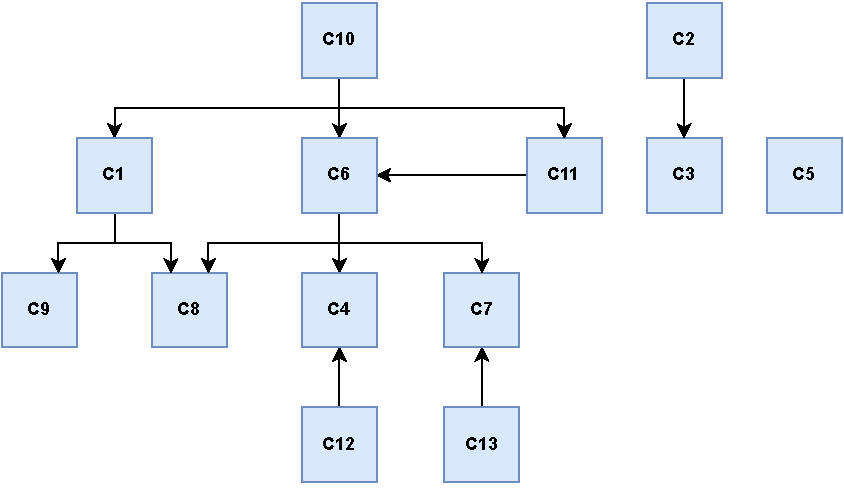
\includegraphics[width=0.87\linewidth]{figures/concept2concept.pdf}
    \caption[Dependencies between Conceptual Models]{Dependencies between
        Conceptual Models (Section~\ref{sec_conceptual})}
    \label{fig:conceptualdependencies}
\end{figure}
\vspace*{\fill}

\vspace*{\fill}
\begin{figure}[tbh]
    \centering
    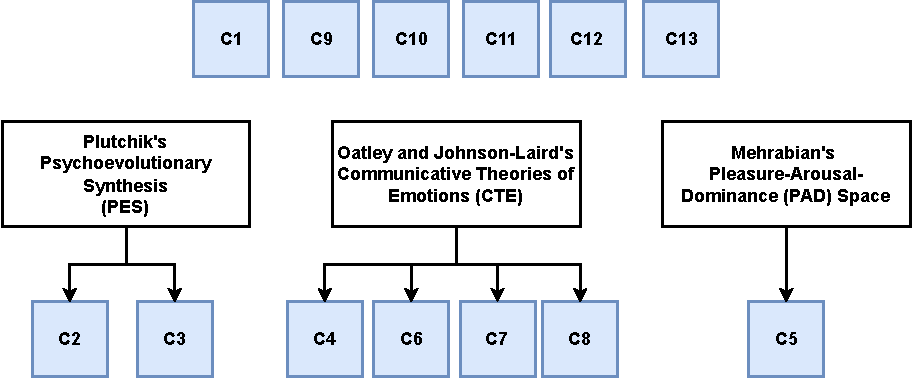
\includegraphics[width=\linewidth]{figures/theories2concept.pdf}
    \caption[Conceptual Model Dependencies on Affective
    Theories/Models]{Conceptual Model Dependencies on Affective Theories/Models
    (Section~\ref{sec_conceptual})}
    \label{fig:theories2conceptual}
\end{figure}
\vspace*{\fill}

\begin{figure}[tbh]
    \centering
    \includegraphics[height=0.96\textheight]{figures/assumptions2All.pdf}
    \caption[Dependencies on Assumptions]{Dependencies on Assumptions (Orange)
    (Section~\ref{sec_assumptions})}
    \label{fig:A2All}
\end{figure}

\begin{landscape}
    \begin{figure}[tbh]
        \centering
        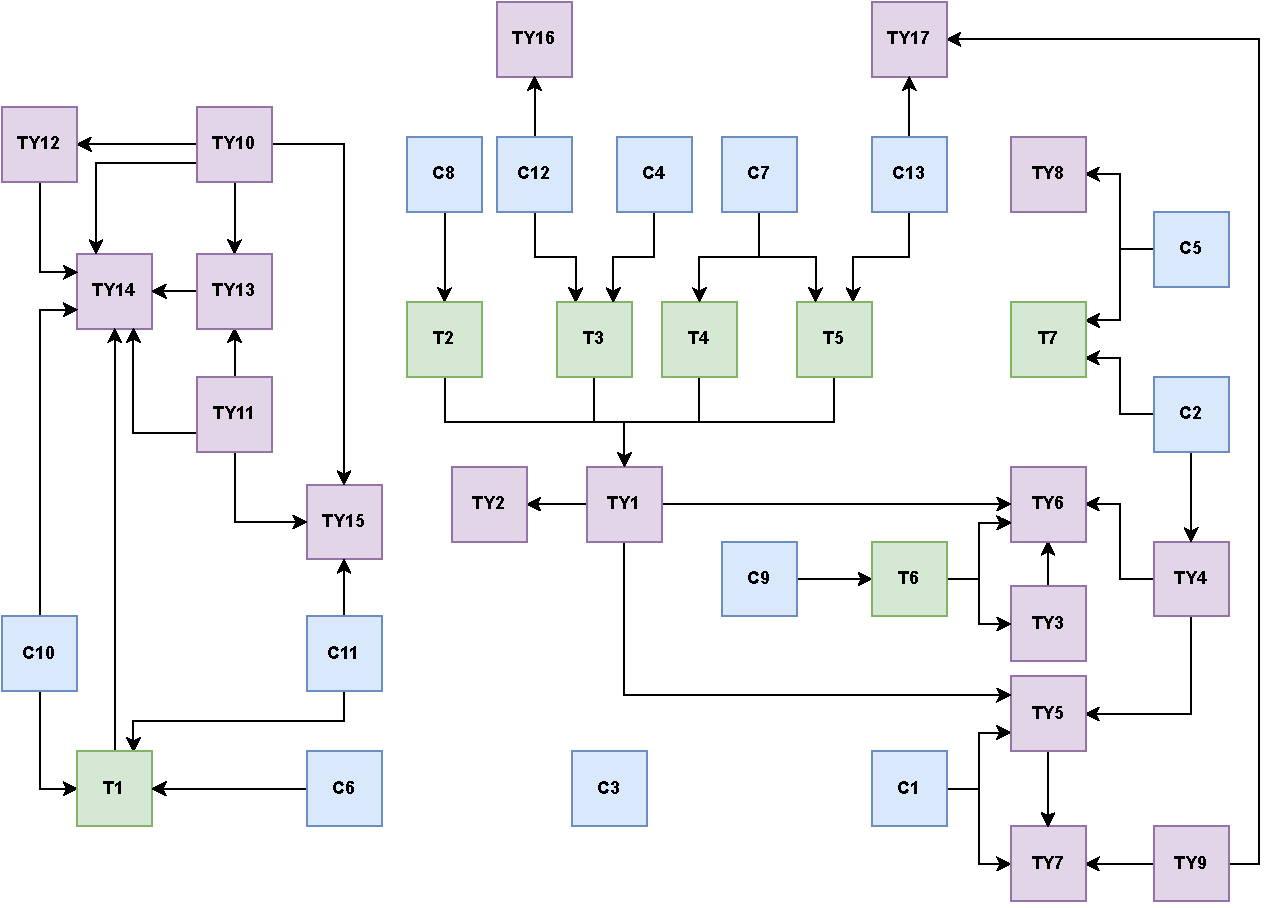
\includegraphics[width=\linewidth]{figures/concept2types_revised.pdf}
        \caption[Traceability between Theoretical Models and Data Types, and
        their dependencies on Conceptual Models]{Traceability between
        Theoretical Models (Green) and Data Types (Purple), and their
        dependencies on Conceptual Models (Blue)
        (Sections~\ref{sec_theoretical}, \ref{sec_typedefs},
        and~\ref{sec_conceptual})}
        \label{fig:C2TY}
    \end{figure}
\end{landscape}

\begin{landscape}
    \begin{figure}[tbh]
        \centering
        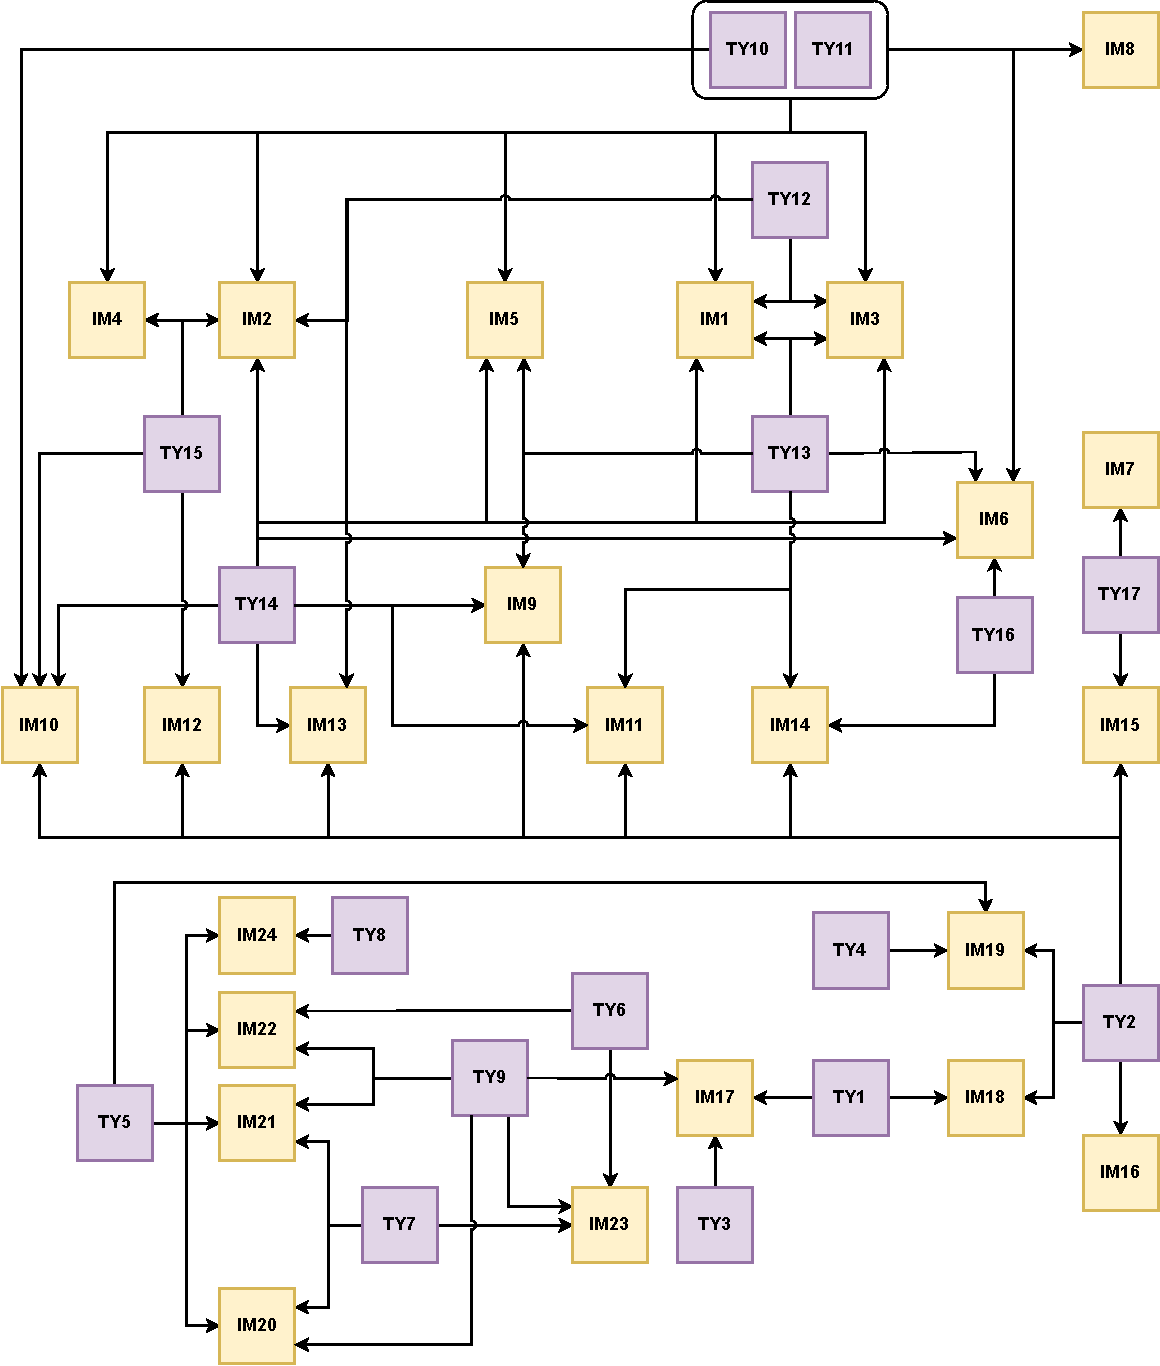
\includegraphics[width=0.88\linewidth]{figures/types2instance.pdf}
        \caption[Instance Models and their Dependencies on Theoretical Models
        and Data Types]{Instance Models (Yellow) and their Dependencies on
        Theoretical Models (Green) and Data Types (Purple)
        (Sections~\ref{sec_theoretical}, \ref{sec_typedefs},
        and~\ref{sec_instance})}
        \label{fig:T-TY2IM}
    \end{figure}
\end{landscape}

\vspace*{\fill}
\begin{figure}[tbh]
    \centering
    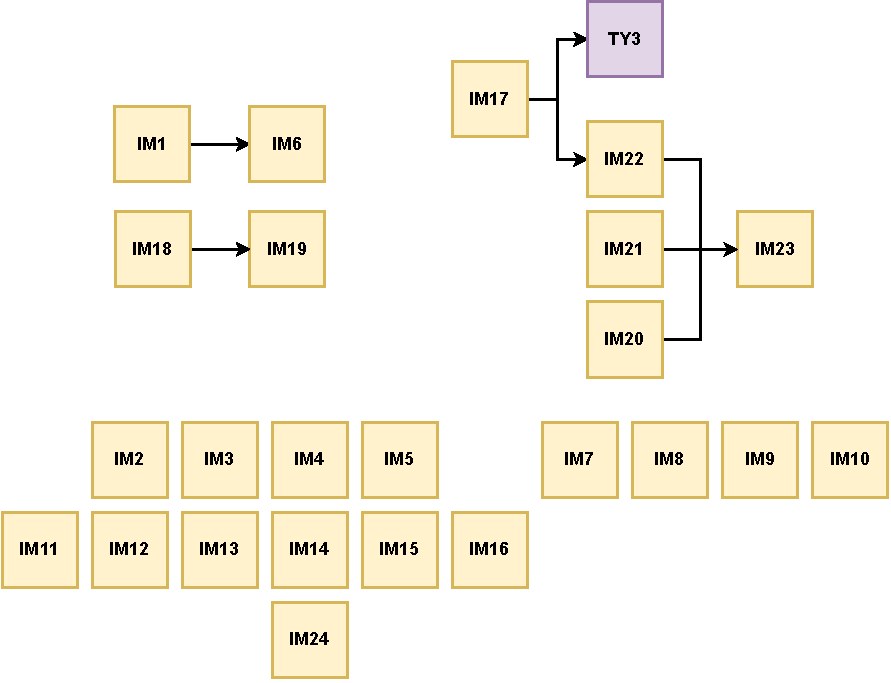
\includegraphics[width=0.5\linewidth]{figures/instance2instance.pdf}
    \caption[Dependencies between Instance Models]{Dependencies between
        Instance Models (Section~\ref{sec_instance})}
    \label{fig:IM}
\end{figure}
\vspace*{\fill}

\begin{figure}[tbh]
    \centering
    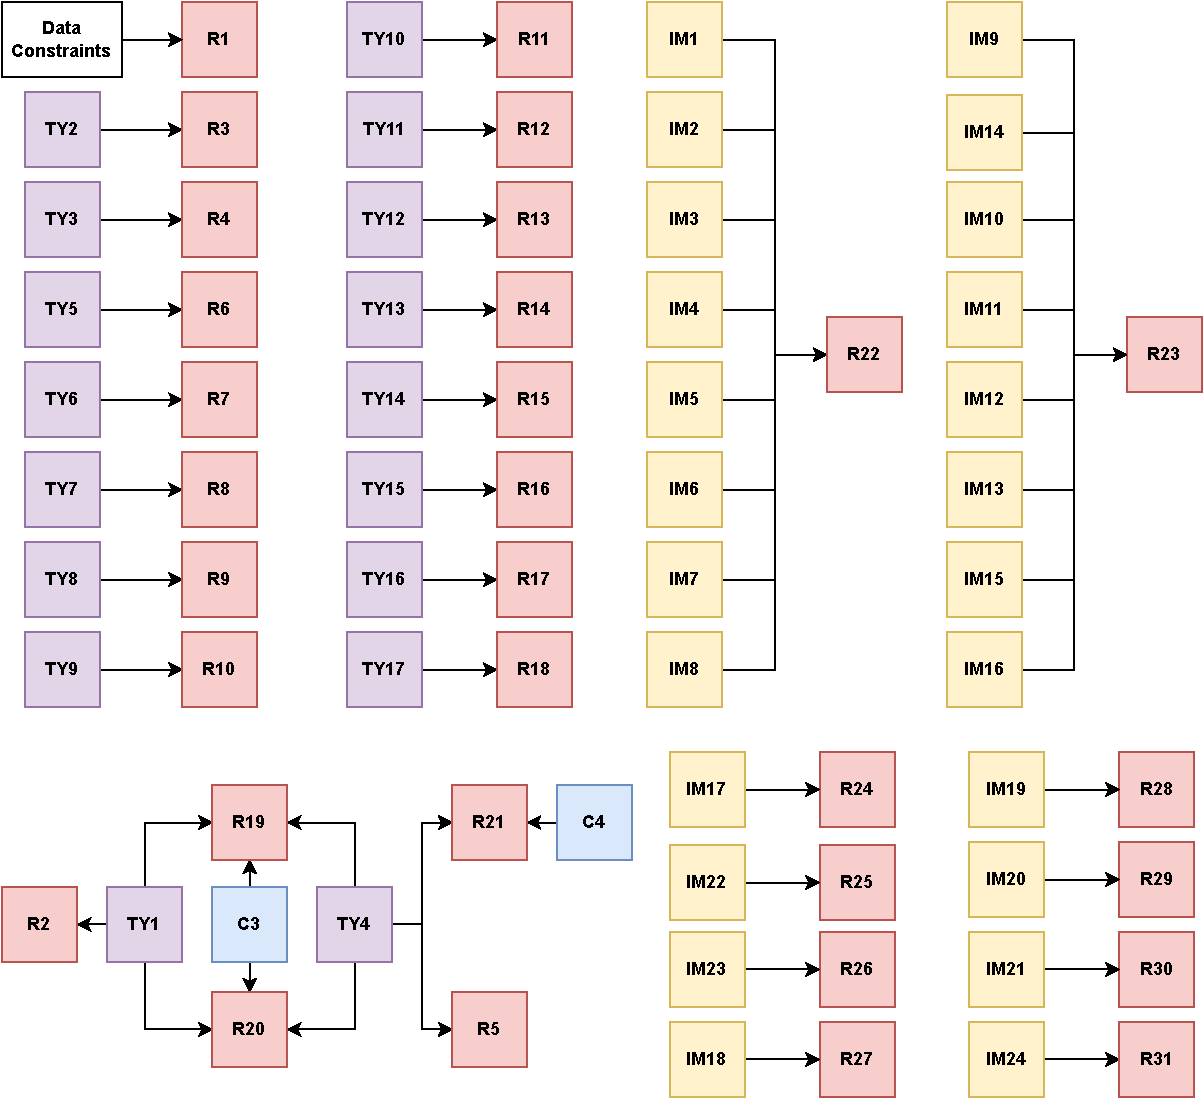
\includegraphics[width=\linewidth]{figures/reqs2All.pdf}
    \caption[Functional Requirements and their Dependencies on Conceptual
    Models, Data Types, Instance Models, and Data Constraints]{Functional
    Requirements (Red) and
    their Dependencies on Conceptual Models (Blue), Data Types (Purple),
    Instance Models (Yellow), and Data Constraints
    (Sections~\ref{sec_conceptual}, \ref{sec_typedefs}, \ref{sec_instance},
    \ref{sec_DataConstraints}, and \ref{sec_functionalreqs})}
    \label{fig:M2R}
\end{figure}

    \clearpage

    \section{Use Hierarchy Between Modules}\label{SecUse}

\citet{Parnas1978} said of two programs, A and B, that A {\em uses} B if the
correct execution of B might be necessary for A to complete the task as
specified. That is, A {\em uses} B if there exist situations in which the
correct functioning of A depends upon the availability of a correct
implementation of B.

The \textit{uses} hierarchy between modules (Figure~\ref{FigUH}) shows that the
graph is a directed acyclic graph (DAG). Each level of the hierarchy offers a
testable and usable subset of the system. Modules in the higher level of the
hierarchy are simpler because they use modules from the lower levels.

\vspace*{\fill}
\begin{figure}[!tbh]
    \centering
    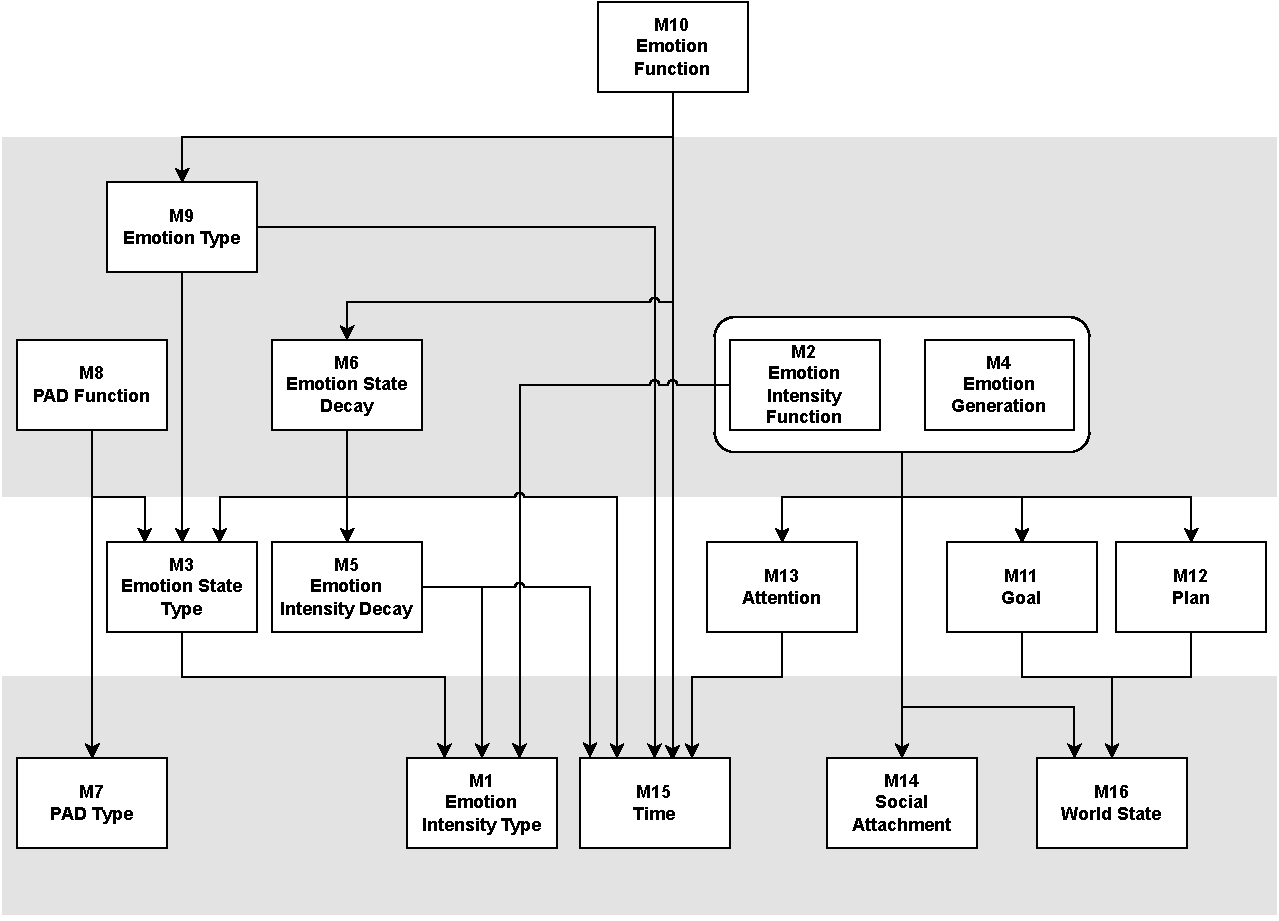
\includegraphics[width=\linewidth]{figures/usesHierarchy.pdf}
    \caption{Use hierarchy among modules}
    \label{FigUH}
\end{figure}
\vspace*{\fill}

    \clearpage

    \bibliographystyle{ACM-Reference-Format}
    \bibliography{../../../refs/references_documentation,
    ../../../refs/references, ../../../refs/references_gamedesign,
    ../../../refs/references_SEPerspective, ../../../refs/references_psych}

\end{document}